
\begin{infocard}{Volumen de un prisma recto}
    \begin{wrapfigure}{r}{0.3\textwidth }
        \centering
            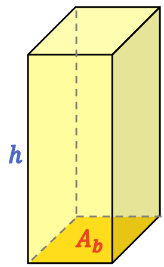
\includegraphics[width=\linewidth]{../images/20230319192423}
        \end{wrapfigure}
    El volumen de un prisma recto de altura $h$, y cuyo polígono base tiene un área $A_b$, es:
    \[  V = A_b h\]
    Si el polígono base es un polígono regular, entonces:
    \[   V  = \dfrac{nLah}{2}\]
    donde $P$ es el perímetro; $a$, la apotema; $n$, el número de
    lados y $l$, la medida del lado.
\end{infocard}



